\section{Introduction}
Replacing Monday with Tuesday in ``The current day is Monday.'' changes the input to a frozen language model and, consequently, its hidden representation. A linear map can be fitted to predict the transformed representation from the original one. The interesting question is whether one map works across all seven weekdays and across different contexts. The prescribed one-day shift also has a known composition rule: seven shifts return to the original state. If fitted maps predict these changes accurately and approximately respect their composition, what structure have we recovered?

Transformation fitting provides a way to investigate this question in fixed representations \citep{lenc2015understanding,sun2026transformationlaws}. Equivariant learning approaches instead learn coordinates together with the transformations that act on them \citep{schmidt2025equivariance}. In either setting, predictive success must be interpreted relative to what was fitted and what was observed. A useful predictor need not attain the best risk in a constrained action class. Nor does a consistently realizable action establish that its specified semantic correspondence is preferred to other coherent correspondences. These distinctions matter even with familiar, explicitly labeled states: a stable category code can support accurate transformations without revealing how the model computes an answer.

We separate three questions. The first is predictive: how well does a fitted operator predict a transformed state in a held-out context? The second concerns an entire class: what is the minimum error attainable by any exact orthogonal action of the prescribed group in a fixed real dimension? The third compares registrations: does the prescribed action on state labels have a larger spectral budget than legitimate alternatives? Figure~\ref{fig:evaluation-targets} shows how these questions branch from the same representation bank. They share observations, but differ in their targets, constraints and evidence.

Our theoretical result addresses the second question. We relate its class optimum to the representation energy that can be captured in a group-invariant subspace under a real-dimension budget. The budget must select complete irreducible components: a two-dimensional rotation component cannot be retained one coordinate at a time. This extra information matters. Two observation systems can have the same optimal unconstrained linear risk and ordinary orbit spectrum, yet different exact-action risks. A type-constrained spectral budget yields lower and upper bounds whose ratio is at most two. The result connects established invariant-approximation and representation-theoretic tools to a specific prediction target; it does not propose another fitting algorithm.

We apply the bound to weekday cycles and square-corner symmetries in six frozen Llama and Qwen models. The observed banks support accurate predictors and yield quantitative bounds on the cost of requiring exact orthogonal actions. Separating independent orthogonality from common group laws reveals substantial heterogeneity: in the primary sixteen-dimensional weekday panel, almost the entire further-law lower-bound sum comes from one condition. That concentration describes the guaranteed lower endpoints, not the unknown exact costs. The prescribed registration has uniquely highest spectral budget in only 7/24 weekday and 16/24 corner conditions, with different counts at dimension eight. Compatibility with an action therefore coexists with condition-dependent preference among alternatives.

The held-out comparisons ask what these fitted structures predict beyond their construction data. Exact actions constructed from training contexts lose to independent least squares in every evaluated test condition, although their action constraints hold under the numerical checks. In a separate authored-context bank, directly fitting context differences improves weekday transport but worsens corner transport relative to coordinate fitting. Together, the results provide a class-risk bound, a quantitative characterization of its costs in frozen representations, and registration comparisons that expose dependence on the observation space. The transport results locate an additional predictive boundary; they do not replicate the spectral comparisons on new contexts or establish native causal computation.

% Keep the three research questions before this figure in the rendered reading order.
\begin{figure}[!hb]
\centering
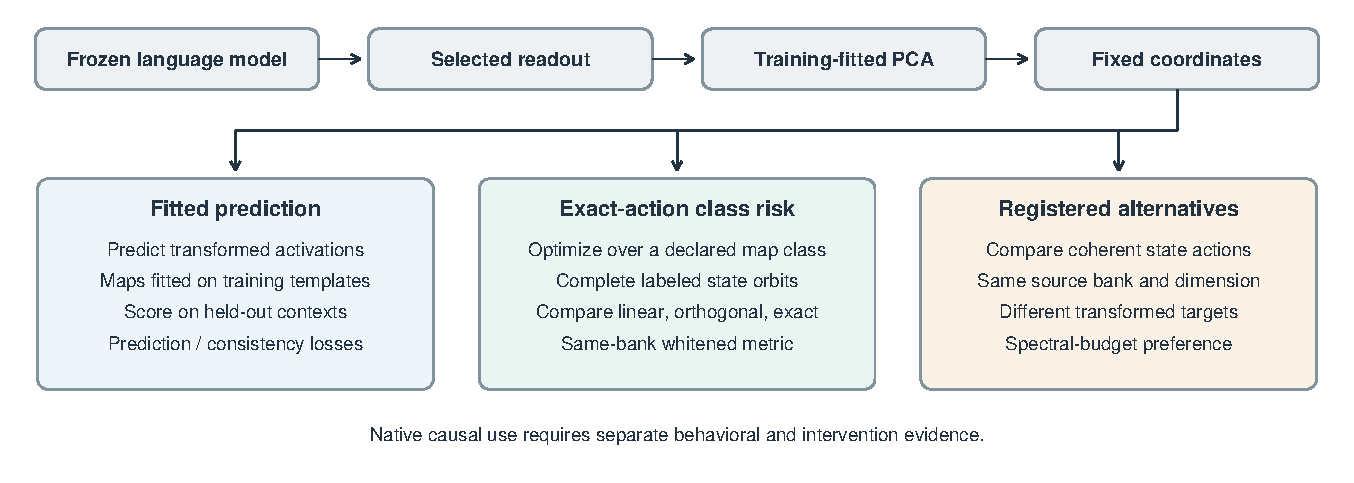
\includegraphics[width=\textwidth]{figures/evaluation_targets.pdf}
\caption{Three questions from the same fixed representations. Fitted prediction evaluates learned maps on held-out contexts; exact-action analysis bounds an optimum in a declared class and metric; registration comparisons change the coherent target action while keeping the source bank fixed. The parallel branches are not a chain of implications toward semantic or causal identification.}
\label{fig:evaluation-targets}
\end{figure}
